As publicações foram analisadas e categorizadas, conforme mostra na Tabela \ref{tab:categorizacao}. As questões de pesquisa foram utilizadas para nortear um caminho a ser percorrido para alcançar o objetivo deste trabalho. A seguir será mostrada uma análise sobre categoria.

\subsection{Tomada de Decisões}

O cérebro humano possui diferentes formas de reconhecimento, duas delas podem ser exemplificadas como experiências subjetivas, tais como o senso de familiaridade e o senso da experiência. O primeiro é uma intuição fraca a uma crença convincentemente forte. O segundo é voltada a lembrança, o que envolve a recuperação de associações entre fatos, requisitando palavras ou ações para que o cérebro dê uma resposta.

Essas duas experiências no entendo, não podem ser ditos ao certo se os dois sensos são processados pelo cérebro de maneiras diferentes. De uma forma geral, a familiaridade é processada mais rapidamente em consideração a experiência. Por exemplo, quando uma pessoa passa por uma atividade que a ela já é comum, a requisição sobre o cérebro é menor do que comparado com a experiência, onde o cérebro necessita de um tempo maior para processar a situação sobre fatos que são ou não conhecidos por ele. 

A tomada de decisões é feita a partir de informações de memória armazenadas em regiões do cérebro, para tanto é necessário um mecanismo para a integração entre as informações neurais distribuídas \cite{buzsaki}. Este mecanismo provavelmente utilizará sinais do hipocampo,este que é considerada a principal sede de memória, para a representar a memória de eventos anteriores \cite{eichenbaum}.

A tomada de decisões pode ser feita a partir de habilidades cognitivas, como a memória, que lhes permitem aprimorar suas decisões. Segundo o filósofo \cite{aristoteles}, “O homem é um animal social por natureza”. Seguindo o pensamento do filósofo, os animais tomam decisões são adaptáveis conforme o grupo em que se encontra. Ao observar esse contexto, é esperado que atitudes tenham decisões diferentes de acordo com a situação. Esse processo de adaptação se baseia de acordo com experiências anteriores, sejam elas senso familiares ou senso de experiência.

Este modelo foi proposto como resultado de pesquisas sobre como o cérebro utiliza de diferentes tipos de experiência para uma tomada de decisão. Essa atitude pode ser tomada a partir de um fator como familiar ou por experiências cotidianas. A velocidade de processamento das informações depende do quão a atividade é exercida pela pessoa, o que leva o cérebro a tratar-las de modo mais rápido ou não. Como a tomada de decisão é exercida a partir de informações armazenadas no cérebro, os neurocientistas possuem um papel muito importante para auxiliar os pesquisadores de tecnologias que visam aprimorar ações de seres que podem ser construídos, como robôs.

\subsection{Inteligência Artificial}

Segundo \cite{anthes}, a Inteligência Artificial (IA) é uma tecnologia com potencial permanente. Como advento de suas descobertas, IA trouxe benefícios como reconhecimento de fala, automação da navegação de veículos, para níveis quase humanos.

Ainda segundo \cite{anthes}, especialistas na área de Inteligência Artificial afirmam que essa tecnologia pode permitir que sistemas sejam inteligentes ao ponto de entender e reagir ao mundo de um ponto de visto humano. 

\cite{john}, afirma que a aprendizagem pode ser vista no sentido biológico como um processo de internalização que detecta, lembra e reproduz sequências bem sucedidas. Resultados de aprendizado ao executar uma ação ou possivelmente várias ações ao mesmo tempo sem esforço cognitivo ou pensamento, ou seja, sem envolvimento consciente.

O hardware de memória é projetado para aprender ações repetidas, sendo feita uma analogia ao aprendizado humano. Ações comuns são mapeadas na memória e podem ser executadas sem esforço da CPU (análogo ao pensamento). Propriedades de IA para sequências mapeadas na memória estão na tabela \ref{tab:artificial}.

\begin{table}[H]
\centering
\begin{tabular}{|c|c|}
\hline
1 & A result of rehearsal                    \\ \hline
2 & Occurs within long term memory \\ \hline
3 & Enables long term modification of underlying circuitry \\ \hline
4 & Permits action without CPU effort \\ \hline
5 & Permits action without CPU delays \\ \hline
6 & Permits action without CPU memory usage \\ \hline
7 & Independent sequences may run concurrently \\ \hline
\end{tabular}
\caption{Artificial Learning}
Fonte: \cite{john}
\label{tab:artificial}
\end{table}

Para melhor enfatizar a tabela \ref{tab:artificial}, ela será traduzida para a língua portuguesa brasileira a seguir:

\begin{table}[H]
\centering
\begin{tabular}{|c|c|}
\hline
1 & Um resultado do ensaio                    \\ \hline
2 & Ocorre dentro da memória de longo prazo \\ \hline
3 & Permite a modificação a longo prazo dos circuitos subjacentes \\ \hline
4 & Permite ação sem esforço da CPU \\ \hline
5 & Permite ação sem atrasos de CPU \\ \hline
6 & Permite ação sem uso de memória da CPU \\ \hline
7 & Sequências independentes podem ser executadas simultaneamente \\ \hline
\end{tabular}
\caption{Aprendizado Artificial}
Fonte: \cite{john} com Adaptações
\label{tab:artificialtraduzido}
\end{table}

\begin{figure}[H]
		\centering
		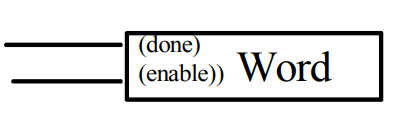
\includegraphics[width=14.5cm]{figuras/sinaisdememoria}
        \caption{Símbolo para uma palavra de memória de longo prazo com controles}
        Fonte: \cite{john}
		\label{img:palavra}
\end{figure}

Para entender a Figura \ref{img:palavra}, deve se entender primeiro o que é uma memória a longo prazo. Esta memória é a capacidade de se manter uma informação recente de poucos dias ou até décadas. Se difere da memória a curto prazo, pois esta pode armazenar elementos por uns 20-30 segundos.

Nesse contexto, a memória a longo prazo pode ser uma ou um conjunto de palavras, que emitem sinais e comandos quando acionadas, ativando o \textit{enable}, como visto na Figura \ref{img:palavra}. Para o aprendizado de algo que está sendo praticado, é necessário um filtro de tempo para detectar uma repetição ou sequência \cite{john}. Para exemplificar este comportamento, imagine um filtro que detecte sempre que uma determinada palavra é ativada após outra palavra dada é feita. A repetição ou sequência dessa palavra seguida de uma ordem é apreendida pela memória e assim armazenada.

Nesse viés, a IA utiliza dados como entrada e esses dados repetidos, por exemplo palavras, são armazenadas como memórias a longo prazo. Essas memórias, usa do princípio inicial da Inteligência Artificial de aprender conforme a inserção dos dados e responder conforme esses dados. Seguindo essa lógica, tem-se o advento do aprendizado de máquina recorrente de dados externos, no caso da IA, e conforme a inserção de mais dados, maiores e mais diferentes serão as atitudes que serão realizadas por ela.